\documentclass[11pt,a4paper]{article}

\usepackage{../../templates/style}

\begin{document}

\begin{problem}{Domino}{standard input}{standard output}{1 second}{16 megabytes}

มีโดมิโน $N$ ชิ้นวางเรียงอยู่บนเส้นแนวแกน $x$ ที่วางตามแนวซ้าย-ขวา  จุดปลายด้านซ้ายของเส้นถือว่ามีพิกัดในแกน $x$ เท่ากับ $0$ เราจะเรียกโดมิโนเรียงตามลำดับจากปลายด้านซ้ายไปยังปลายด้านขวา โดยเริ่มจากชิ้นที่ $1$ ไปจนถึงชิ้นที่ $N$ โดมิโนชิ้นที่ $i$  มีความสูง $H_i$ และวางอยู่บนเส้นที่มีพิกัดแกน $x$ เท่ากับ $X_i$  ตัวอย่างการวาง (ในแนวด้านข้าง) แสดงดังรูป

\begin{figure}[h]
\centering
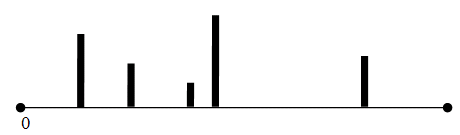
\includegraphics[width=0.7\textwidth]{../latex/img/1052/1052-1.png}
\end{figure}

ในการเล่นโดมิโนนั้น  เราจะเลือกโดมิโนตัวแรกแล้วผลักไปทางด้านซ้ายหรือทางด้านขวาก็ได้  ถ้าโดมิโน “ล้ม” ไปโดนโดมิโนตัวใด  ตัวที่ถูกล้มโดนจะล้มไปชนตัวอื่น ๆด้วย โดมิโนสามารถล้มออกไปนอกขอบของเส้นตรงด้านล่างได้

อย่างไรก็ตาม เราถือว่าโดมิโนไม่มีความหนา  ดังนั้นถ้าล้มไปแล้วปลายโดมิโนไปสัมผัสอีกตัวหนึ่งพอดี จะไม่มีการล้มต่อ  ยกตัวอย่างเช่น ถ้ามีโดมิโนความสูง $1$ หน่วยอยู่ที่ตำแหน่ง $10$ และมีโดมิโนอีกชิ้นอยู่ที่ตำแหน่ง $11$ ถ้าโดมิโนความสูง $1$ หน่วย ถูกทำให้ล้มไปทางด้านขวา โดมิโนที่อยู่ที่ตำแหน่ง $11$ จะไม่ล้มไปด้วยเพราะว่าไม่มีการชน (โดมิโนที่ล้มลงมาสัมผัสอีกอันพอดี)


\bigskip
\underline{\textbf{โจทย์}}  จงเขียนโปรแกรมรับข้อมูลของโดมิโน จากนั้นให้คำนวณหาโดมิโนตัวตั้งต้นที่เราควรจะไปผลัก (จะเป็นการผลักไปทางซ้ายหรือทางขวาก็ได้)  เพื่อทำให้มีโดมิโนล้มลงมากที่สุด


\InputFile

\textbf{บรรทัดแรก} ระบุจำนวนเต็ม $N$ $(1 \leq N \leq 100\,000)$  

\textbf{บรรทัดที่ $2$ ถึง $N+1$} แต่ละบรรทัดจะระบุข้อมูลของโดมิโนแต่ละอัน กล่าวคือ บรรทัดที่ $i+1$  จะระบุข้อมูลของโดมิโนชิ้นที่ $i$ โดยจะระบุจำนวนเต็มสองจำนวน  $X_i$  $H_i$ $(1 \leq  X_i \leq 1\,000\,000\,000; 1 \leq H_i \leq 1\,000\,000\,000)$  รับประกันว่า  $0 \leq X_i < X_i+1$  สำหรับทุก ๆ  $1 \leq i < N$
\newpage

\OutputFile

\textbf{มีบรรทัดเดียว }ประกอบไปด้วยจำนวนเต็ม $J$ และอักขระ $D$ โดยที่ $J$ คือหมายเลขของโดมิโนที่ถ้าเราเริ่มผลัก และอักขระ $D$ จะเป็นค่า "L" หรือ "R" เพื่อระบุทิศทางในการผลัก โดยที่ "L" แทนการผลักไปทางซ้าย และ "R" แทนการผลักไปทางขวา  ถ้ามีโดมิโนหลายชิ้นที่พลักได้จำนวนเท่ากัน ให้ตอบตัวที่มีหมายเลขน้อยที่สุด  และในกรณีที่พิจารณาโดมิโนตัวที่มีหมายเลยน้อยที่สุดแล้วผลักได้ทั้งสองทิศทาง ให้ตอบการผลักไปทางซ้าย

\Examples

\begin{example}
\exmp{5
1 1
3 3
5 4
7 15
10 3}{2 R}%
\end{example}

\Scoring

\textbf{ไม่น้อยกว่า 20\% ของข้อมูลชุดทดสอบ}: $N \leq 1\,000$

\Source

สอบปฏิบัติครั้งที่ 2 ค่ายคัดเลือกผู้แทนประเทศไทย ไปแข่งขันคอมพิวเตอร์โอลิมปิกระหว่างประเทศปี 2550 ค่ายที่ 1

\end{problem}

\end{document}